\chapter{Regression Basics for the Slope}

\section{The Regression Model and Why We Need Inference for the Slope}\index{regression slope!inference}

A sleep researcher pulls data from a sample of $8$ teenagers: daily screen time, in hours, and how many hours they slept that night. She plots the points, fits a line, and finds a slope of $b_1 = -0.16$: for every extra hour of screen time, sleep drops by about ten minutes. Does this mean the effect is real across all teenagers, or could a sample this size show a slope like this by chance?

Recall from the Numerical Methods chapter that the \index{least-squares line}least-squares line $\hat{y} = b_0 + b_1x$ describes your sample: descriptive statistics, not inference.

A sample slope $b_1$ estimates an unknown population slope $\beta_1$, the same way $\hat{p}$ estimates $p$ and $\bar{x}$ estimates $\mu$. Statisticians describe the true relationship between two quantitative variables using a \newterm{population regression model}\index{population regression model}:
\[
Y = \beta_0 + \beta_1 X + \varepsilon
\]
$\beta_0$ is the population $y$-intercept, $\beta_1$ is the population slope, and $\varepsilon$ is random error: the part of $Y$ not explained by $X$. $\beta_0$ and $\beta_1$ are parameters, describing the entire population; $b_0$ and $b_1$ are statistics, calculated from your sample, used to estimate them.

The rest of this chapter reasons from $b_1$, the number your sample gives you, to $\beta_1$, the value you actually care about, using the same confidence interval and significance test tools you've already built for proportions and means.

\subsection*{Estimating the Slope and Intercept}

The formulas for $b_0$ and $b_1$:
\[
b_1 = r\frac{s_y}{s_x} \qquad \text{and} \qquad b_0 = \bar{y} - b_1\bar{x}
\]
where $r$ is the sample correlation coefficient and $s_x, s_y$ are the sample standard deviations of $X$ and $Y$. If you are working from raw sums instead of $r$, $s_x$, and $s_y$, an algebraically equivalent formula is
\[
b_1 = \frac{n\sum xy - \left(\sum x\right)\left(\sum y\right)}{n\sum x^2 - \left(\sum x\right)^2}
\]
Both formulas give the same $b_1$. You can use whichever matches the summary statistics you have.

The \index{residual}residual for any data point is still $e = y - \hat{y}$, where $\hat{y} = b_0 + b_1x$ is the value your line predicts. The standard deviation of all the residuals in your sample, $s_e$, tells you the typical size of a prediction miss. You will use $s_e$ heavily, because it is the key in measuring how much $b_1$ itself might vary from sample to sample.

Following the sleep researcher's study, she samples $8$ teenagers at random and records their daily screen time ($X$, in hours) and their sleep duration that night ($Y$, in hours):

\begin{center}
\begin{tabular}{|c|c|c|c|c|c|c|c|c|}
\hline
Screen time (hr) & 2 & 3 & 4 & 5 & 6 & 7 & 8 & 9 \\
\hline
Sleep duration (hr) & 7.85 & 8.05 & 7.40 & 7.55 & 6.90 & 7.35 & 6.70 & 6.95 \\
\hline
\end{tabular}
\end{center}

For this sample, $\bar{x} = 5.5$, $\bar{y} = 7.34$, $s_x = 2.45$, $s_y = 0.47$, and $r = -0.854$. That gives
\[
b_1 = (-0.854)\frac{0.47}{2.45} = -0.165 \qquad b_0 = 7.34 - (-0.165)(5.5) = 8.25
\]
so $\hat{y} = 8.25 - 0.165x$. The negative slope matches what the researcher suspected: more screen time is associated with less sleep, at least in this sample. The question this chapter answers is whether that association is strong enough and consistent enough, to conclude something about $\beta_1$ for teenagers in general, or whether a slope this far from zero is a believable result of sampling variation alone.

\begin{itemize}
    \item $Y = \beta_0 + \beta_1 X + \varepsilon$ is the population regression model; $\beta_0$ and $\beta_1$ are unknown parameters, and $\varepsilon$ is random error.
    \item $b_0$ and $b_1$ are sample statistics, calculated from your data, that estimate $\beta_0$ and $\beta_1$.
    \item $b_1 = r\dfrac{s_y}{s_x}$ and $b_0 = \bar{y} - b_1\bar{x}$, with an equivalent raw-sum formula available for $b_1$.
    \item The residual $e = y - \hat{y}$ and its standard deviation $s_e$ measure how far actual data points fall from the line.
\end{itemize}

\begin{Exercise}[title={Identifying the Model}, label={ex:slope-model-1}]
A horticulturist records the amount of fertilizer applied (in grams per plant) and the resulting plant height (in centimeters) for a random sample of tomato plants.
\begin{enumerate}
    \item Identify $X$ and $Y$ in this study.
    \item Write the population regression model for this relationship, using correct notation.
    \item In context, what would it mean if $\beta_1 = 0$?
    \item Explain why $\beta_1$ is not something the horticulturist can ever know exactly, even after collecting data from every plant she owns.
\end{enumerate}
\end{Exercise}

\begin{Answer}[ref={ex:slope-model-1}]
\begin{enumerate}
    \item $X$ is the amount of fertilizer applied (grams per plant); $Y$ is the resulting plant height (centimeters).
    \item $Y = \beta_0 + \beta_1 X + \varepsilon$, where $\beta_0$ is the population intercept, $\beta_1$ is the population slope relating fertilizer amount to height, and $\varepsilon$ is random error.
    \item If $\beta_1 = 0$, then fertilizer amount has no linear relationship with plant height in the population; the population regression line is flat, and knowing how much fertilizer a plant received tells you nothing about how tall it will grow.
    \item $\beta_1$ describes the relationship for the entire population of plants the horticulturist could ever grow, under all possible conditions, not just the ones she happened to collect data from. Even collecting data from every plant she currently owns would still leave $\beta_1$ unknown, since her plants are themselves a sample of all plants that could exist under those growing conditions. $\beta_1$ is a parameter; only a $b_1$ calculated from data is ever directly observed.
\end{enumerate}
\end{Answer}

% \begin{Exercise}[title={Spot the Error}, label={ex:slope-model-2}]
% A student in the sleep study writes: "I calculated $\beta_1 = -0.165$ from my sample of 8 teenagers, so I can conclude that increasing screen time by one hour causes a decrease of $0.165$ hours of sleep for every teenager." Identify two separate errors in this statement.
% \end{Exercise}
%
% \begin{Answer}[ref={ex:slope-model-2}]
% First, the value $-0.165$ was calculated from the sample, so it should be labeled $b_1$, not $\beta_1$. $\beta_1$ refers to the unknown population slope; $b_1$ is the sample statistic used to estimate it. Second, the statement claims causation from an observational study. Unless screen time was randomly assigned to teenagers in an experiment, a relationship in the data does not establish that screen time causes reduced sleep. Other variables, such as stress or extracurricular schedules, could be influencing both screen time and sleep.
% \end{Answer}
%
% \begin{Exercise}[title={Computing the Line}, label={ex:slope-model-3}]
% An engineer records the operating temperature (in degrees Celsius) and the battery life (in hours) for a random sample of $6$ devices. She finds $\bar{x} = 30$, $\bar{y} = 9.2$, $s_x = 8.5$, $s_y = 1.4$, and $r = -0.79$.
% \begin{enumerate}
%     \item Find $b_1$ and $b_0$.
%     \item Write the least-squares regression equation.
%     \item Predict the battery life for a device operating at $35^\circ$C.
% \end{enumerate}
% \end{Exercise}
%
% \begin{Answer}[ref={ex:slope-model-3}]
% \begin{enumerate}
%     \item $b_1 = (-0.79)\dfrac{1.4}{8.5} = -0.130$; $b_0 = 9.2 - (-0.130)(30) = 13.10$.
%     \item $\hat{y} = 13.10 - 0.130x$.
%     \item At $x = 35$: $\hat{y} = 13.10 - 0.130(35) = 8.55$ hours.
% \end{enumerate}
% \end{Answer}

\textbf{Computing in Excel}

Enter the sleep study data from earlier in this section into two columns: screen time in cells A2 through A9, and sleep duration in cells B2 through B9, with headers in row 1.

\begin{enumerate}
    \item In an empty cell, enter \texttt{=SLOPE(B2:B9,A2:A9)}. Excel returns $-0.1649$, matching $b_1 = -0.165$ from the hand calculation (Excel simply keeps more decimal places).
    \item In another cell, enter \texttt{=INTERCEPT(B2:B9,A2:A9)}. Excel returns $8.2506$, matching $b_0 = 8.25$.
    \item To check the correlation behind the calculation, enter \texttt{=CORREL(A2:A9,B2:B9)}. Excel returns $-0.8536$, matching $r = -0.854$.
    \item To find $s_x$ and $s_y$ directly instead of computing them by hand, use \texttt{=STDEV.S(A2:A9)} and \texttt{=STDEV.S(B2:B9)}. These return $2.4495$ and $0.4732$.
\end{enumerate}

Watch the argument order: for both \texttt{SLOPE} and \texttt{INTERCEPT}, the known $y$-values are listed first, then the known $x$-values. Reversing the two ranges is a common mistake, and it may hand you the wrong sign or a wrong intercept.

% Exercise 3 gave you $\bar{x}$, $\bar{y}$, $s_x$, $s_y$, and $r$ directly rather than raw data, since with only five summary numbers, computing $b_1 = r\frac{s_y}{s_x}$ by hand is just as fast as opening a spreadsheet. \texttt{SLOPE} and \texttt{INTERCEPT} need the original data columns to work; if you had the original $6$ temperature and battery-life pairs instead, entering them into two columns and applying \texttt{SLOPE} and \texttt{INTERCEPT} directly would skip the $r$, $s_x$, $s_y$ step entirely.

\begin{figure}[H]
    \centering
    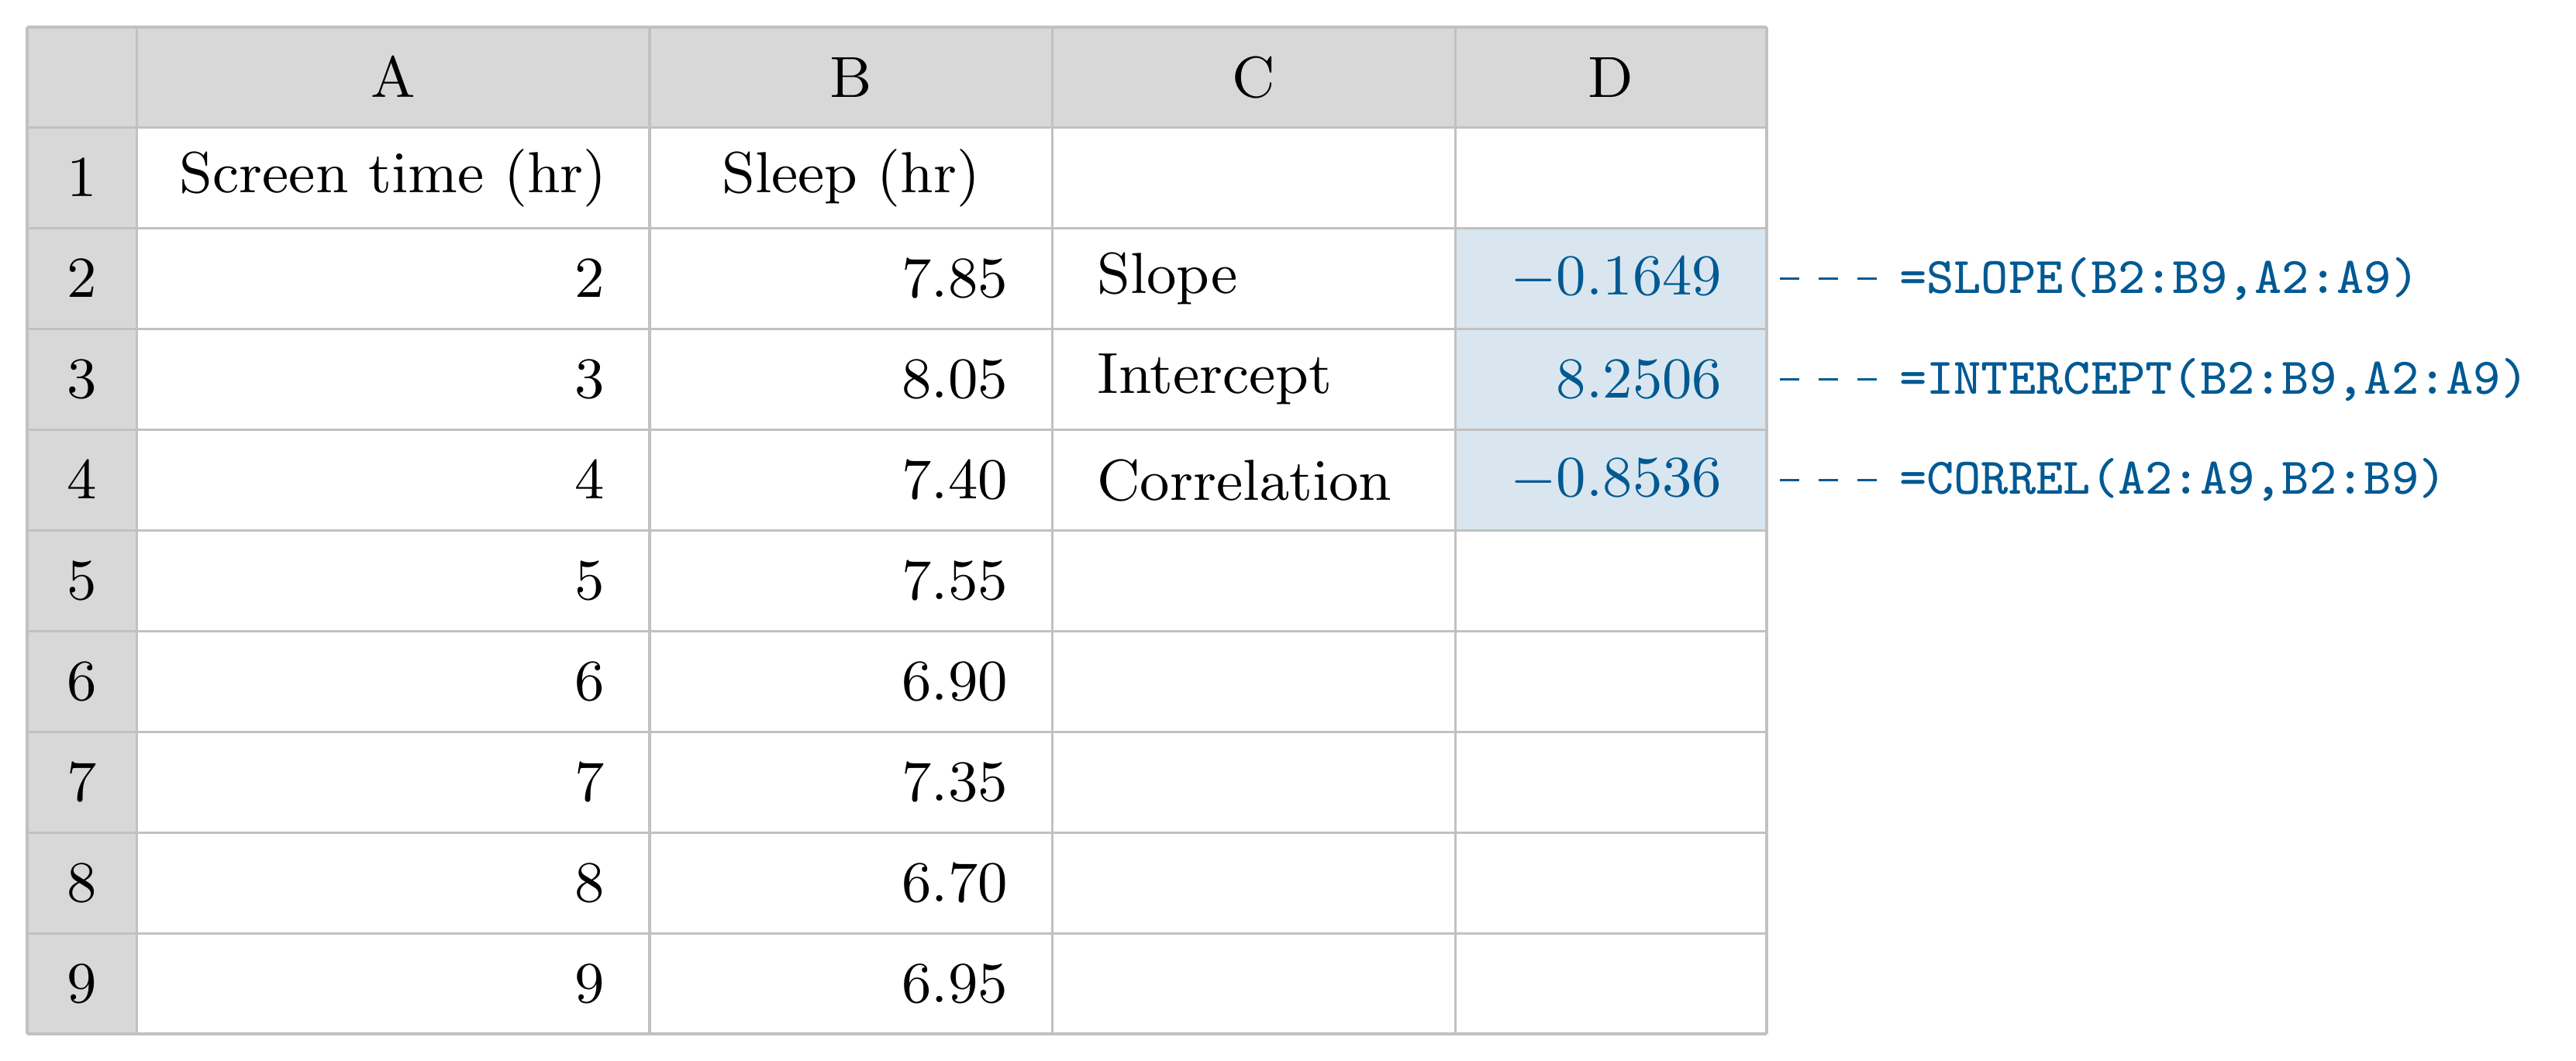
\includegraphics[width=0.84\textwidth]{slope_sheet_coef.png}
    \caption{Spreadsheet layout for the sleep study: data in columns A and B, with each formula beside the result it returns in column D.}
    \label{fig:slope-sheet-coef}
\end{figure}
